\chapter{Desarrollo hardware del manipulador}
\label{cap:capitulo5}

\vspace{1cm}

En este capítulo se aborda el desarrollo necesario para, a partir de un concepto, acabar construyendo un prototipo real funcional. Se 
hace incisión en cada etapa necesaria para este cometido.


Escribe aquí un párrafo explicando brevemente lo que vas a contar en este capítulo. En este capítulo (y quizás alguno más) es donde, por fin, describes detalladamente qué has hecho y qué experimentos has llevado a cabo para validar tus desarrollos.

\section{Concepto}
En esta sección se expone como ha sido el proceso de encontrar y definir la idea fundamental del robot, en función de 
los objetivos propuestos, evaluando las distintas opciones para encontrar el que mejor se adapte. Se trata de balance

Primero, se debe conocer el numero de grados de libertad que se ajuste a los requisitos establecidos en la sección \ref{sec:requisitos}. En base 
a los requisitos 1 y 5, que limitan en cuanto a precio de fabricación y complejidad de los mismos, se ha decidido limitar los grados de 
libertad a un máximo de 4. 

hablamos del tipo de joints que existente
Existen muchos tipos de joints entre los que destacan:

\begin{itemize}
\item Revolución: Este tipo de \textit{joint} permite el movimiento de rotación alrededor de un eje fijo. Está restringido a 1 DOF. Es comúnmente usado en todo tipo de robots, sobre todo en industriales.
\item Prismático: En este tipo de \textit{joint}, las partes del robot se pueden desplazar linealmente a lo largo de un eje específico. Está restringido a 1 DOF. Es usado ptincipalmente en 
los carros de avance de robot industriales y en máquinas CNC.
\item Esférico: Esta articulación permite la rotación en cualquier dirección. Está restringido a 3 DOF y suele ser usado como articulación pasiva, es decir, que 
que su movimiento depende de restricciones externas.
\item Cilíndrica: Esta articulación permite el movimiento de rotación alrededor de un eje y también un desplazamiento lineal a lo largo del mismo. Combina los movimientos rotacionales y prismáticos. Está restringido a 2 DOF. Es usado en el extremo de los 
robots tipo \textit{Scara}.

\begin{figure} [h!]
  \centering    
  \subfigure[Revolución]{\label{fig:j_rot}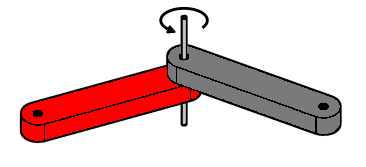
\includegraphics[width=0.3\linewidth ]{figs/joint_rot.png}}
  \hspace{1cm}
  \subfigure[Prismático]{\label{fig:j_prism}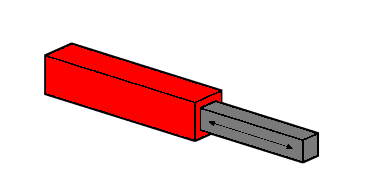
\includegraphics[width=0.3\linewidth]{figs/joint_prism.png}}
  \subfigure[Esférico]{\label{fig:j_esf}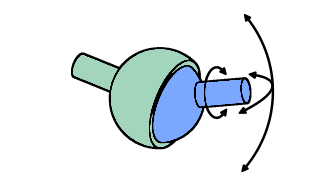
\includegraphics[width=0.3\linewidth ]{figs/joint_esf.png}}
  \hspace{1cm}
  \subfigure[Cilíndrico]{\label{fig:j_cil}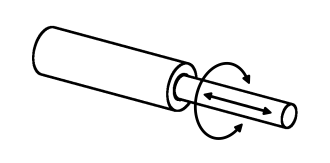
\includegraphics[width=0.3\linewidth]{figs/joint_cil.png}}
  \caption{Tipos de articulaciones más usadas en robótica}
\end{figure}

\end{itemize}


Con hasta 4 grados de libertad podemos realizar los siguientes robots:
Tipos:

\begin{enumerate}
\item Robots \acs{SCARA}: son una categoría de robots industriales ampliamente utilizados en aplicaciones de ensamblaje electrónico, operaciones de 
\textit{pick and place}(coger componentes y situarlos en una determinada posición) y empaquetado de productos, entre otras.
Se caracterizan por su diseño de brazo articulado y su capacidad para realizar movimientos rápidos 
y precisos en un plano horizontal. Este tipo de robot suele tener tres o cuatro grados de libertad, en función de si en el extremo del 
robot puede rotar sobre si mismo o no. 

\begin{figure} [h!]
  \centering    
  \subfigure[Ensamblado de baterías]{\label{fig:fanuc}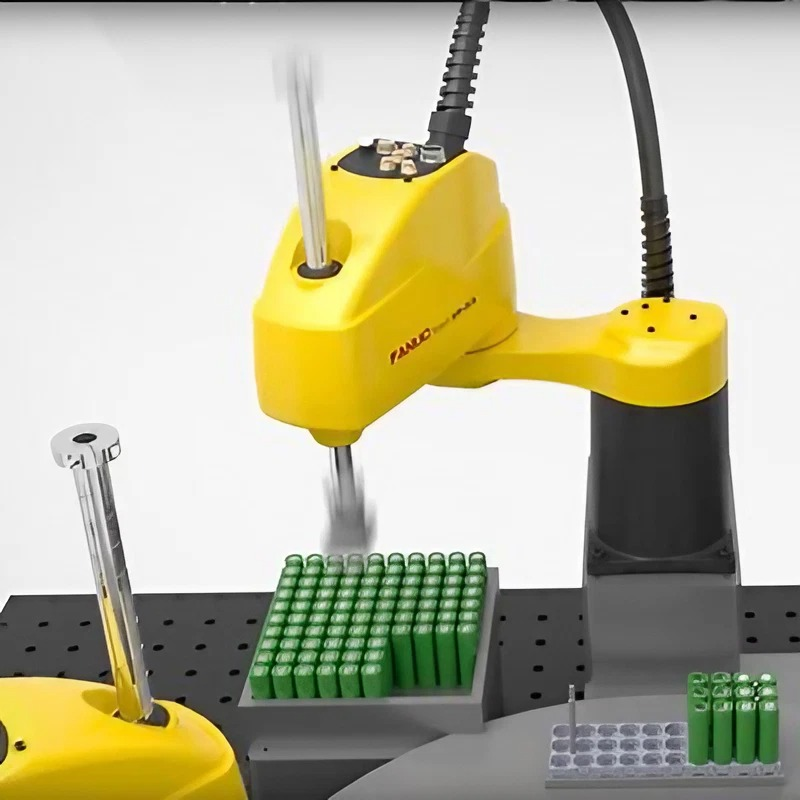
\includegraphics[width=0.3\linewidth ]{figs/fanuc.jpg}}
  \hspace{3cm}
  \subfigure[Espacio de trabajo]{\label{fig:fanuc_ws}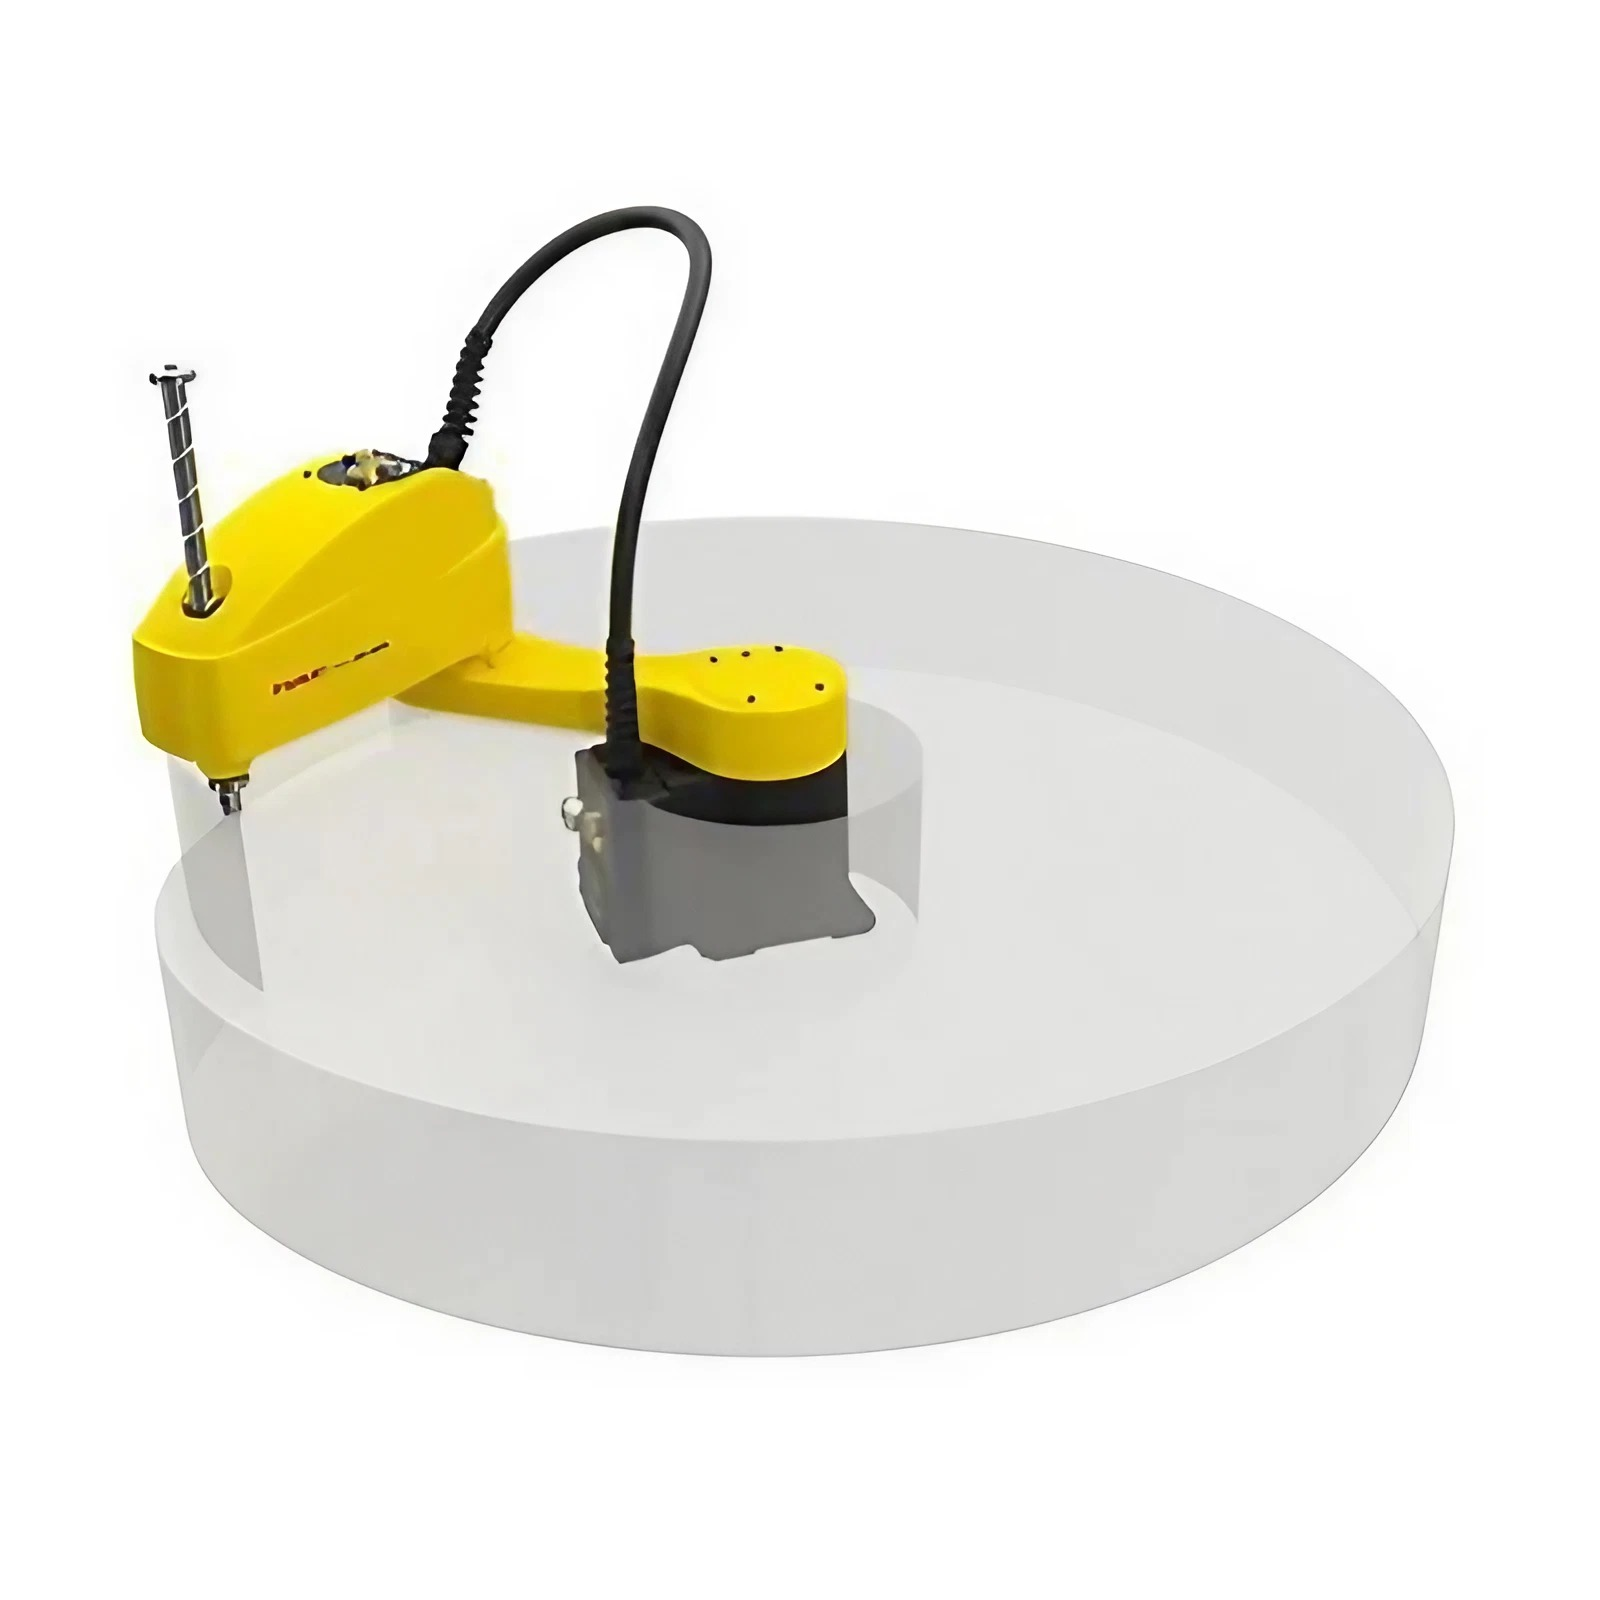
\includegraphics[width=0.3\linewidth]{figs/fanuc_spacio.jpg}}
  \caption[Fanuc SR-3iA]{Ejemplo: FANUC SR-3iA\footnote{\url{https://www.fanuc.eu/uk/en/robots/robot-filter-page/scara-series/scara-sr-3ia}}}
\end{figure}

\item Robots articulados: estos robots tienen una estructura similar a un brazo humano con múltiples articulaciones y ejes rotatorios. Suelen tener entre 4 y 6 ejes y permiten movimientos complejos y flexibles. 
\begin{figure} [h!]
  \centering    
  \subfigure[Robot real]{\label{fig:rebel}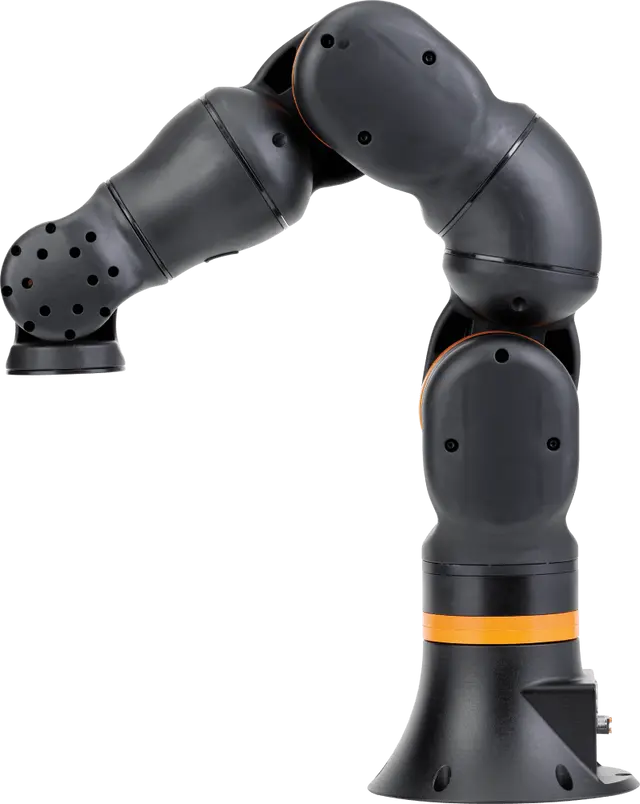
\includegraphics[width=0.3\linewidth ]{figs/rebel4dof.jpg}}
  \hspace{3cm}
  \subfigure[Espacio de trabajo]{\label{fig:rebel_ws}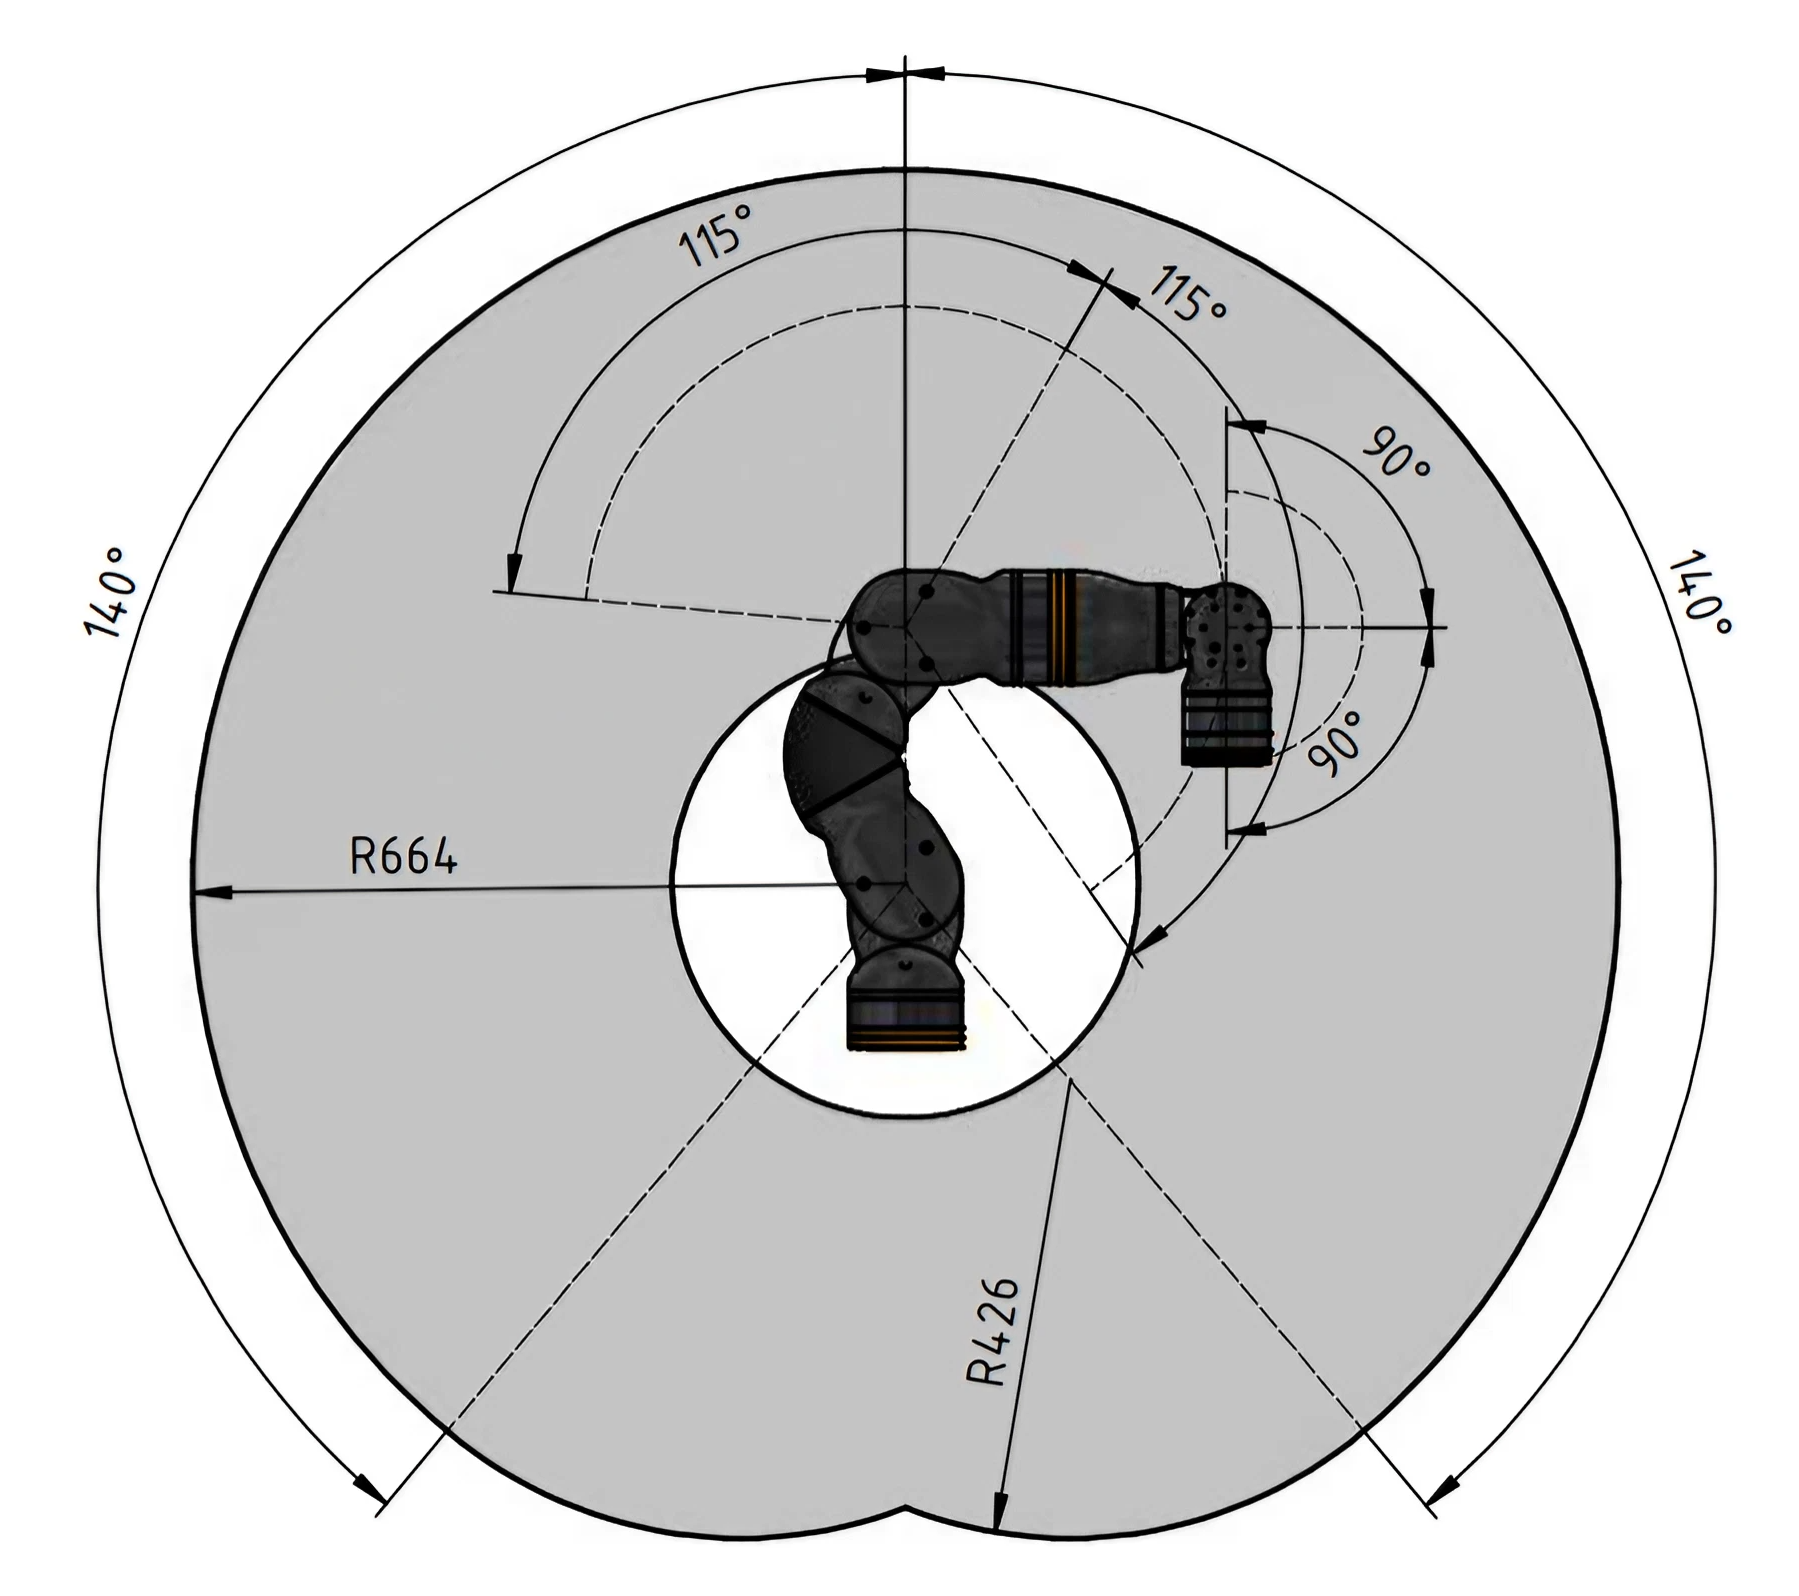
\includegraphics[width=0.4\linewidth]{figs/igus_space.png}}
  \caption[REBEL-4DOF-01]{Ejemplo: REBEL-4DOF-01\footnote{\url{https://www.igus.es/product/20962?artNr=REBEL-4DOF-01}}}
\end{figure}



\item Robots basados en paralelogramos:
\begin{itemize}
\item El robot Delta es un tipo de robot paralelo de 3 (o más) grados de libertad compuesto por dos bases unidas por tres cadenas 
cinemáticas basadas en el uso de paralelogramos. La base superior se encuentra fija mientras la base inferior, donde se 
ubica el efector final, es móvil y siempre está paralela a la base fija.
Son rápidos y precisos, por lo que se utilizan en aplicaciones que requieren alta velocidad, como en la 
industria alimentaria o en la selección y empaquetado de productos.

M-410iC/185 

\begin{figure} [h!]
  \centering    
  \subfigure[Robot Delta ABB]{\label{fig:delta}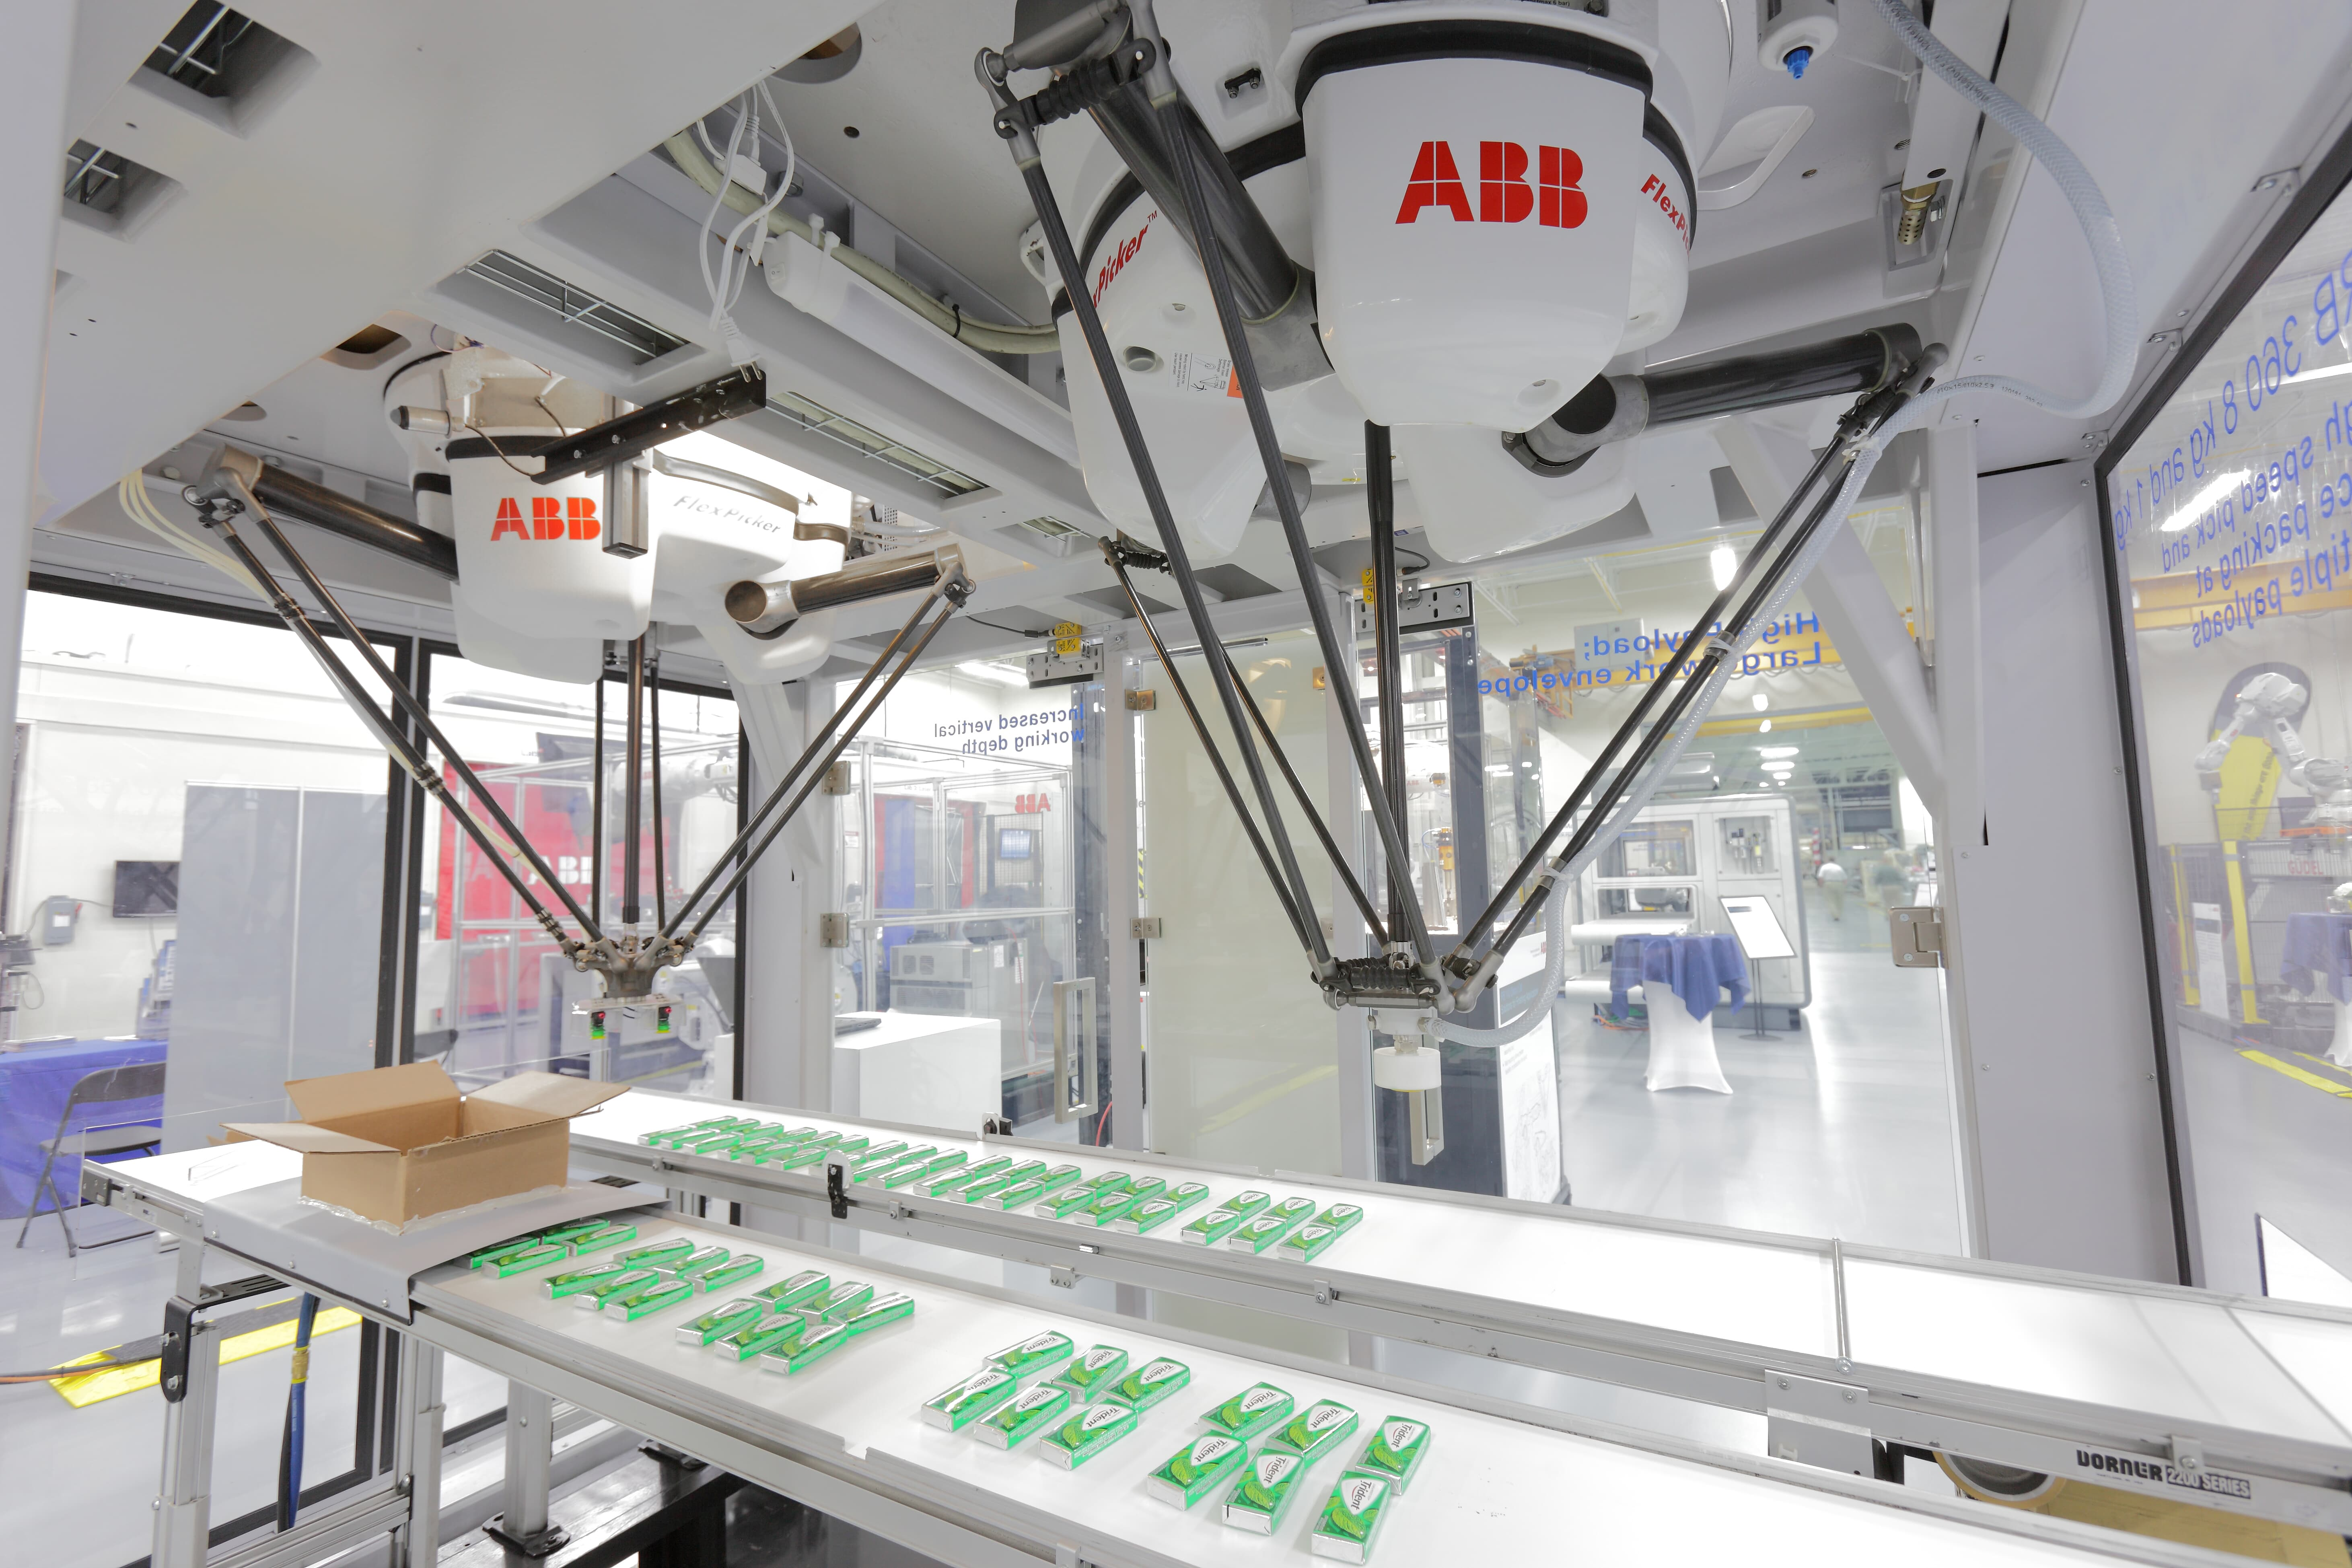
\includegraphics[width=0.3\linewidth ]{figs/delta_flex_picker.png}}
  \hspace{3cm}
  \subfigure[FANUC M-410iC/185]{\label{fig:paral}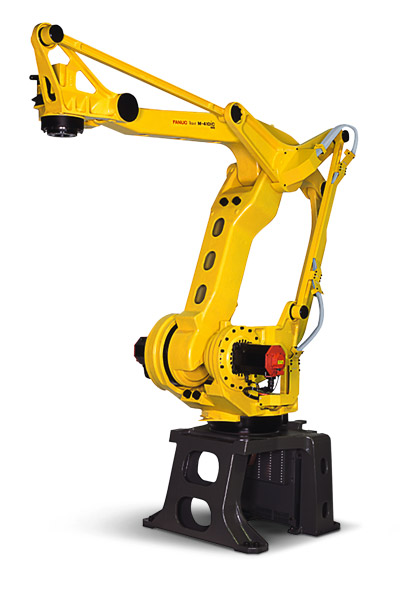
\includegraphics[width=0.3\linewidth]{figs/m_410.jpg}}
  \caption{Robots basados en paralelogramos}
\end{figure}
\end{itemize}

https://www.fanuc.eu/uk/en/robots/robot-filter-page/m-410-series/m-410ic-185

\item Robots cartesianos: se mueven sobre rieles/guías a lo largo de tres ejes cartesianos (X, Y, Z) y cuyos ejes forman ángulos rectos unos respecto de 
los otros. Se trata de un tipo de máquina muy común en la industria.
\begin{figure} [h!]
  \centering    
  \subfigure[VP-2500DP]{\label{fig:pnp}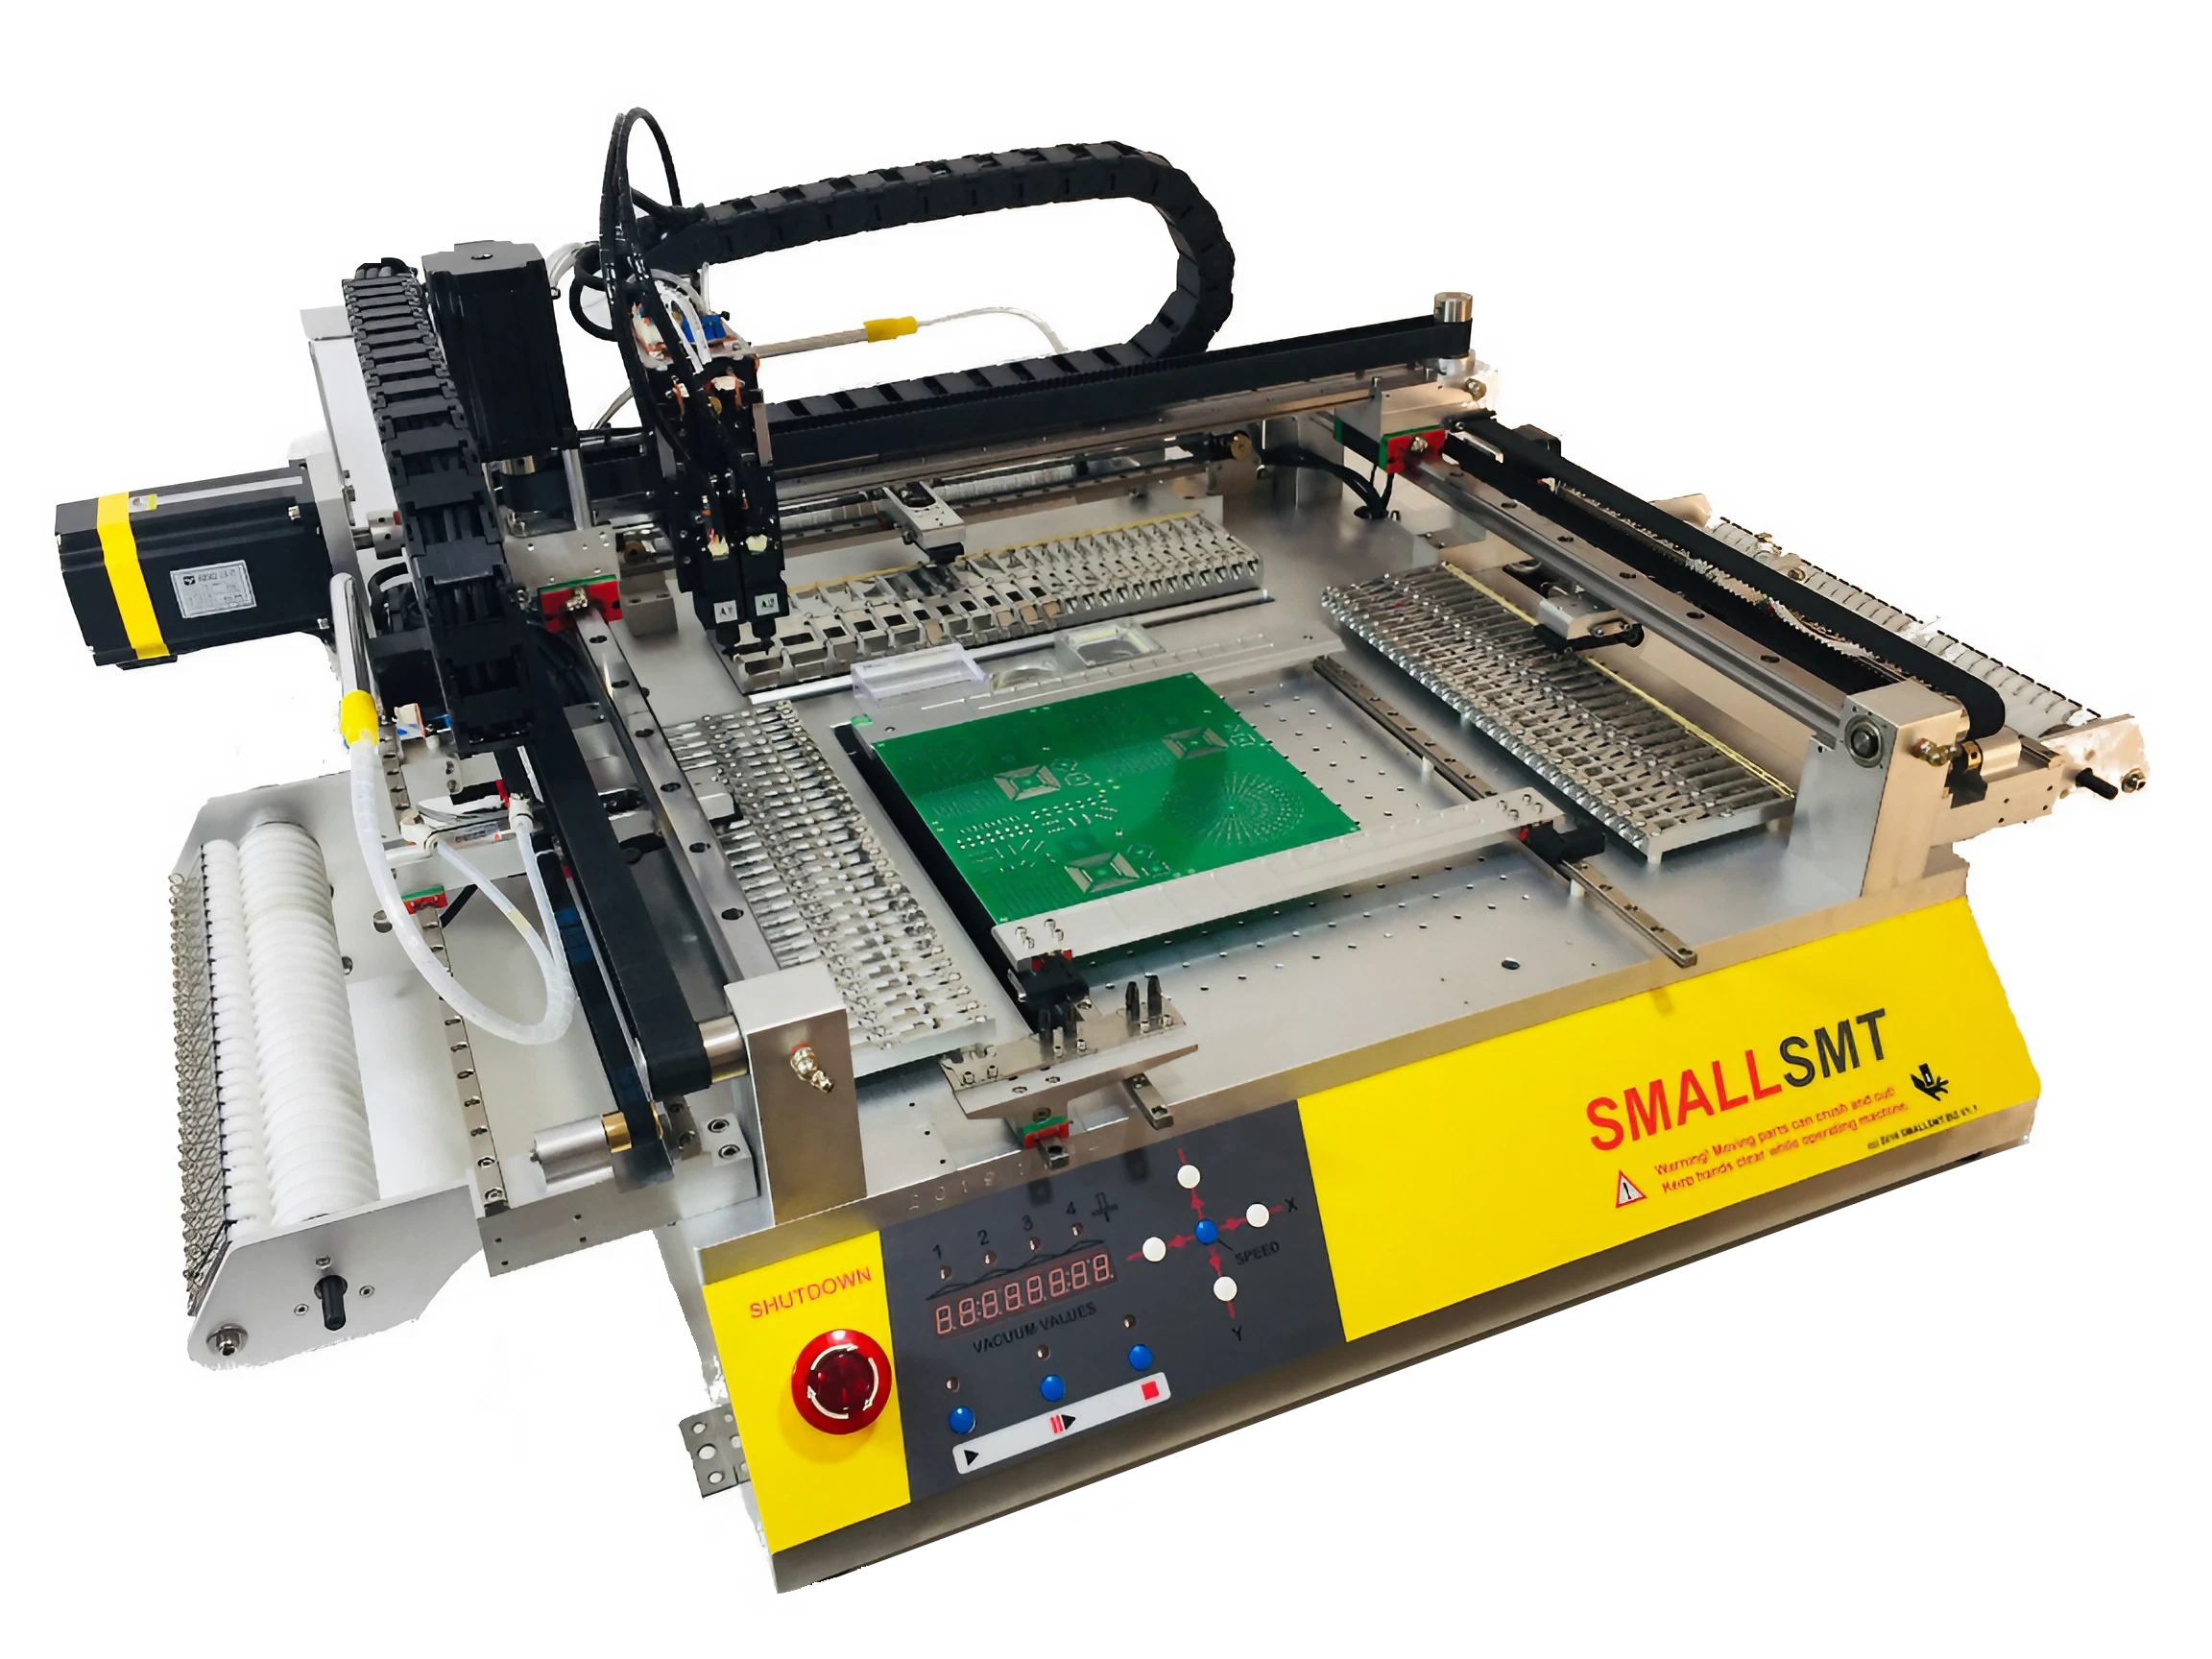
\includegraphics[width=0.4\linewidth ]{figs/pnp.jpg}}
  \hspace{1cm}
  \subfigure[OpenBuilds CNC Lead 1010]{\label{fig:cnc}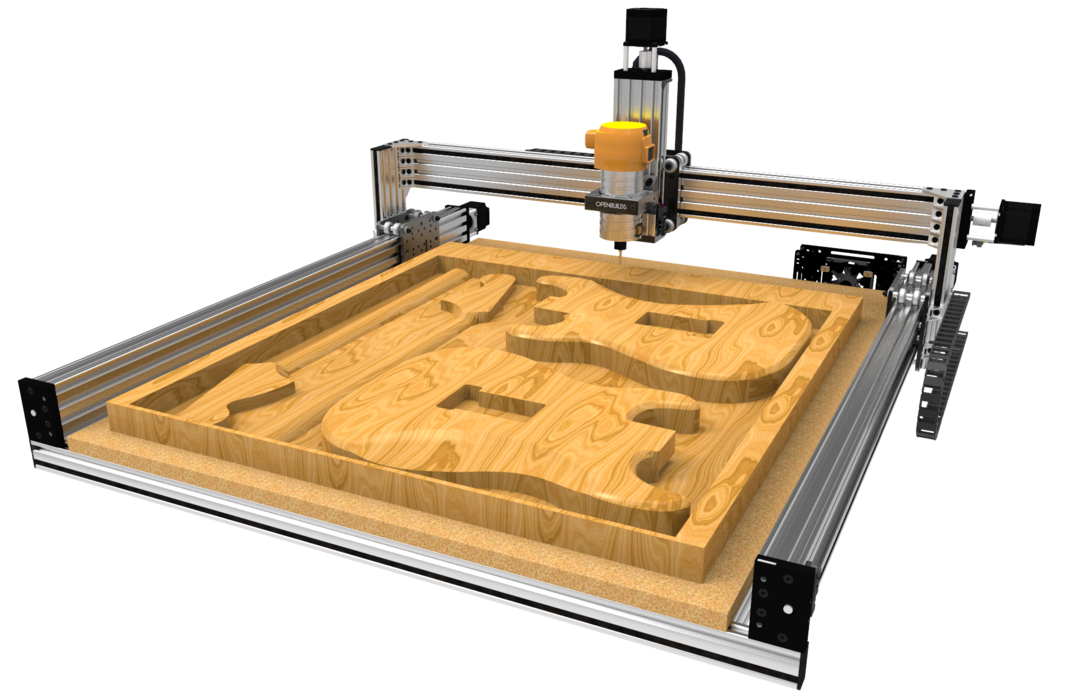
\includegraphics[width=0.4\linewidth]{figs/cnc.jpg}}
  \caption{Ejemplos de robots cartesianos}
\end{figure}

https://openbuilds.com/builds/lead-cnc-1010-40-x-40.7832/

https://www.orion-industry.com/pick-and-place/VP2500DP-WNE-eng.pdf

\end{enumerate}

\section{Modelo alámbrico}
\subsection{En qué consiste}
\label{subsec:eqc_mod_alambrico}
El modelo alámbrico es una forma de analizar el movimiento de un sistema mecánico compuesto por ejes y eslabones. Este 
enfoque simplifica la representación visual al destacar las relaciones espaciales entre las diferentes partes del sistema mediante 
líneas y conexiones simbólicas, en lugar de mostrar detalles realistas del manipulador. 
\begin{figure} [h!]
  \begin{center}
    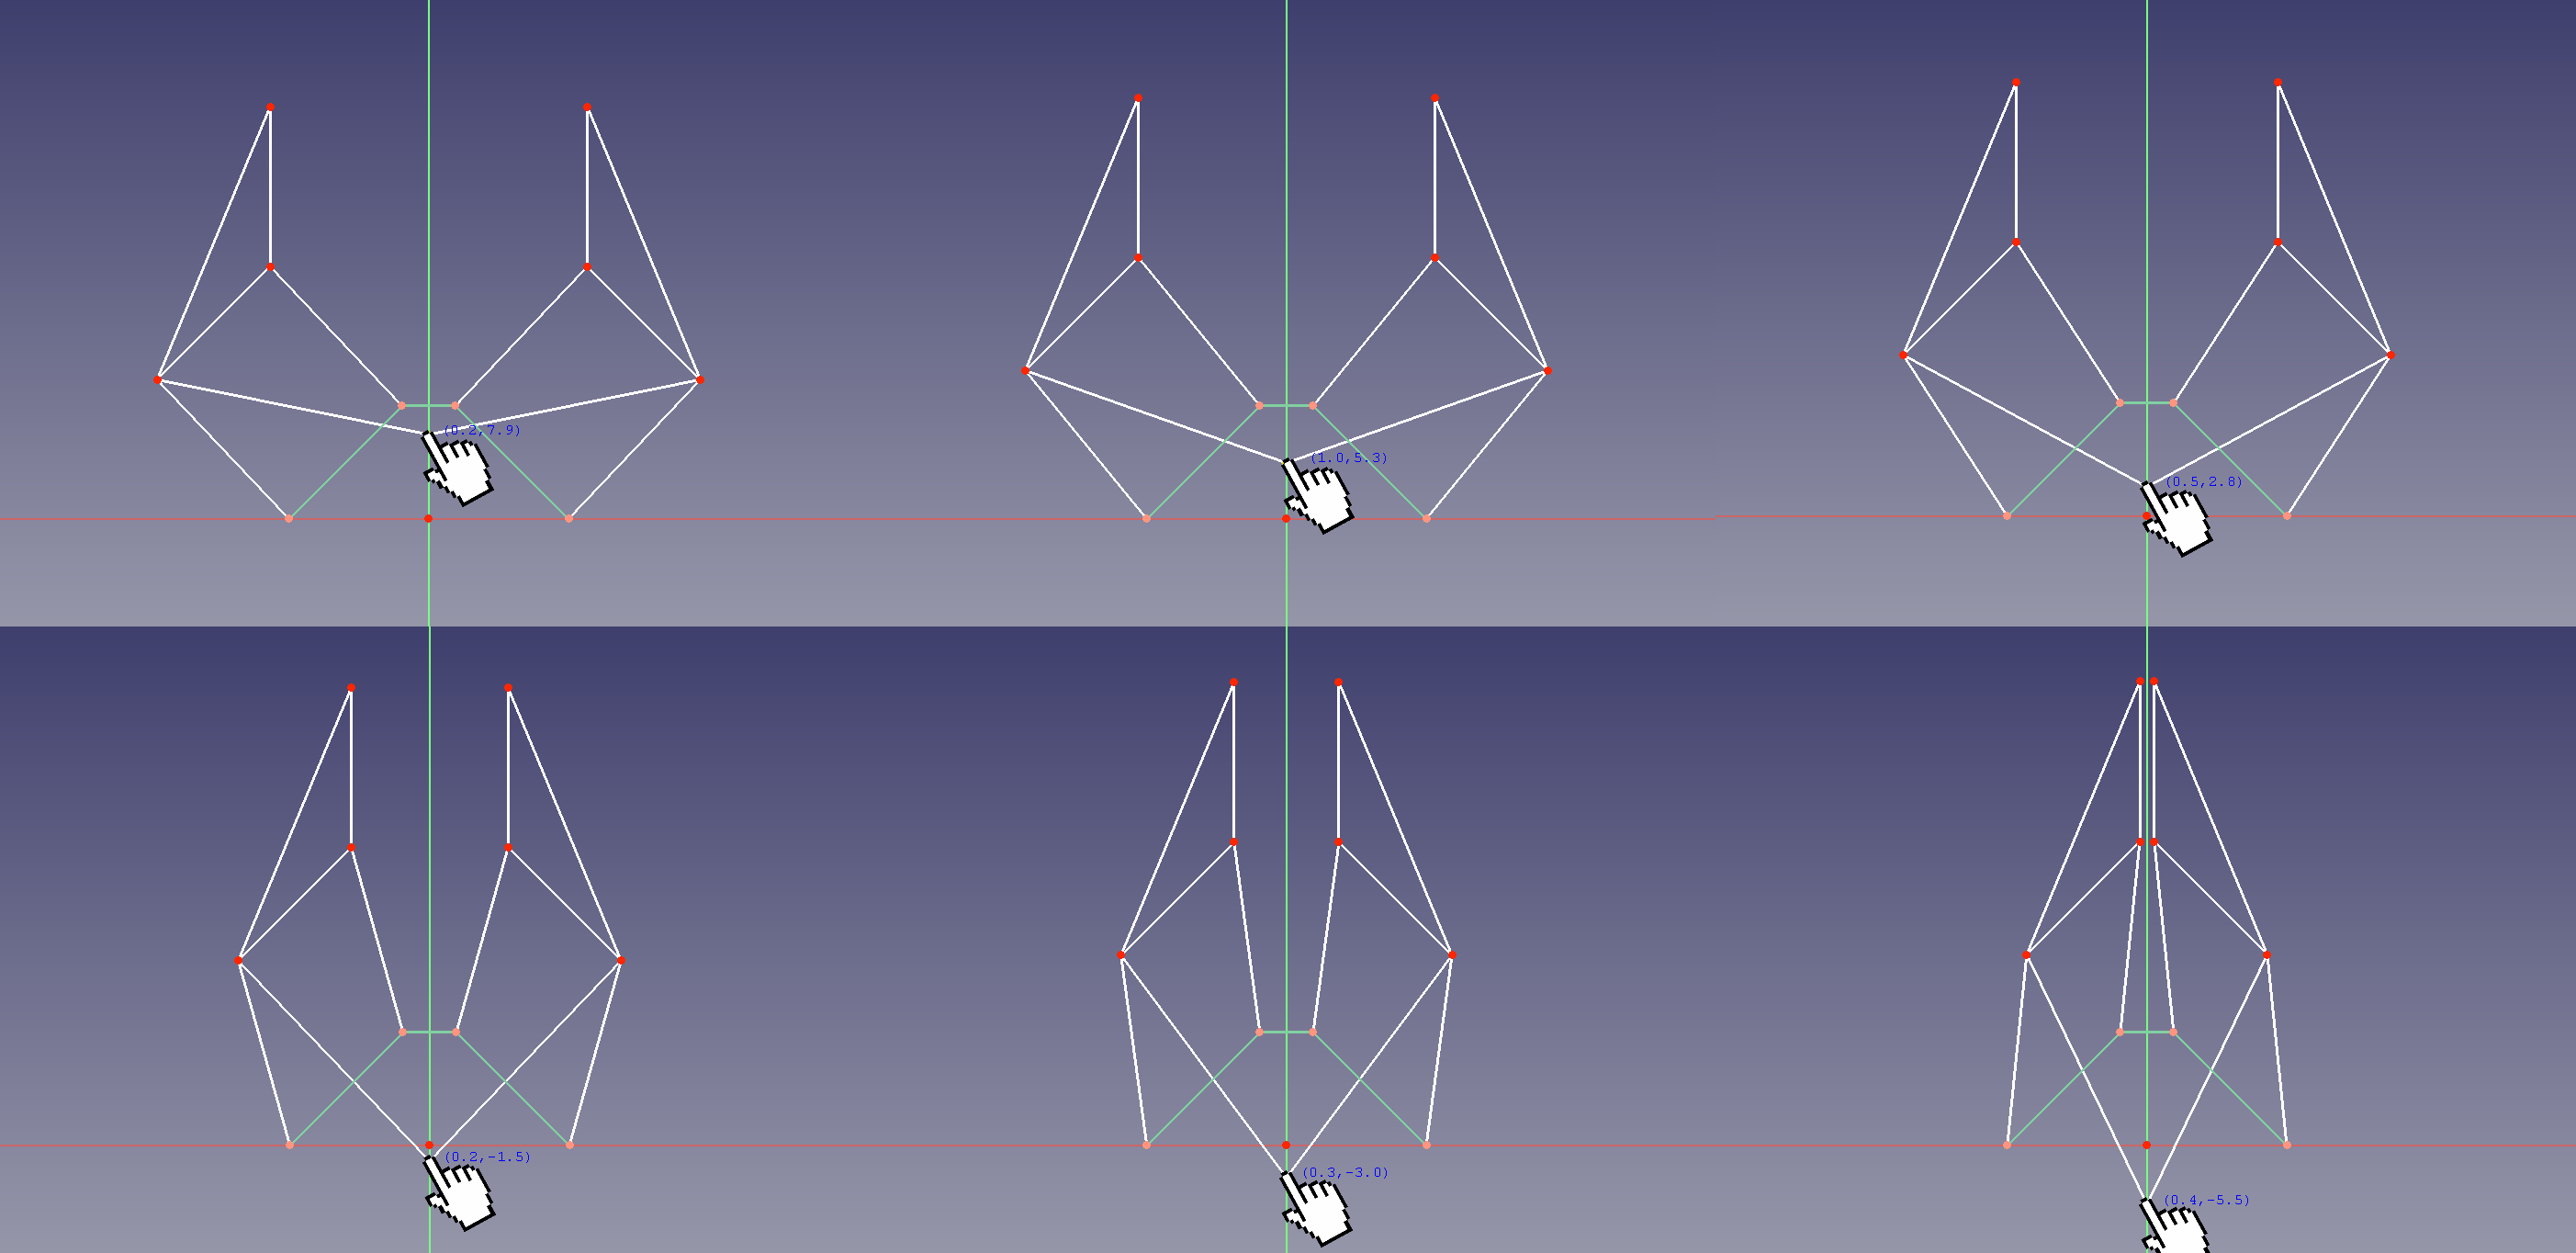
\includegraphics[width=15cm]{figs/pinza_evol.png}
  \end{center}
  \caption{Pinza paralela con 1 grado de libertad}
  \label{fig:mod_pinza_figure}
\end{figure}\ 

\subsection{Modelo alámbrico del brazo MeArm \ref{fig:mearm}}
\label{subsec:mod_mearm}
En esta sección se analiza el comportamiento del modelo alámbrico del manipulador en el que se basa este proyecto.
Está compuesto por una serie de restricciones que definen la dinámica del brazo.


\begin{table}[H]
\begin{center}
\begin{tabular}{|c|c|}
\hline
\textbf{Parámetros} & \textbf{Valores} \\
\hline
L1 & 170mm \\
L2 & 170mm \\
P1 & 35mm \\
P2 & 35mm \\
P3 & 25mm \\
Ángulo P2 & 135º \\
\hline
\end{tabular}
\caption{Parámetros del modelo alámbrico de G-Arm}
\label{cuadro:ejemplo}
\end{center}
\end{table}


\section{Dinámica}



\section{Bocetos}
Una parte importante del diseño son los bocetos previos al modelado 3D. En estos bocetos se busca tener una idea clara de la forma 
y posición de cada pieza, así como de su lugar en el espacio.

\section{Diseño CAD}
En esta sección se va a hablar de las particularidades del diseño y diversas cosas que hay que tener en cuenta a la hora de diseñar 
cualquier pieza mecánica que posteriormente será impresa en plástico. Además se divaga sobre las posibles piezas mecánicas que se 
pueden usar para lograr la mejor relación resultados-precio.
Para el diseño de este brazo robot, se ha utilizado dos herramientas de diseño. Inicialmente el proyecto se realizó mediante 
la herramienta \textit{Fusion 360} y posteriormente se utilizó FreeCad\ref{sec:freecad} para cumplir el objetivo de ser totalmente 
\textit{Open Source} y parametrizado, para que cualquier persona pueda investigarlo, modificarlo y utilizarlo de forma gratuita. 
El diseño 3D se ha ido contruyendo en a partir de los bocetos y modificando ligeramente en función de como iba quedando.


  
\section{Impresión y montaje}
En esta sección se exponen todos los detalles a tener en cuenta a la hora de querer replicar este proyecto. Para la impresión 
de G-Arm se ha utilizado una impresora Ender-3 Pro\footnote{\url{https://www.creality.com/products/ender-3-pro-3d-printer}} y un rollo 
de 1Kg de filamento PLA Rojo convencional.
\begin{figure} [h!]
\begin{center}
  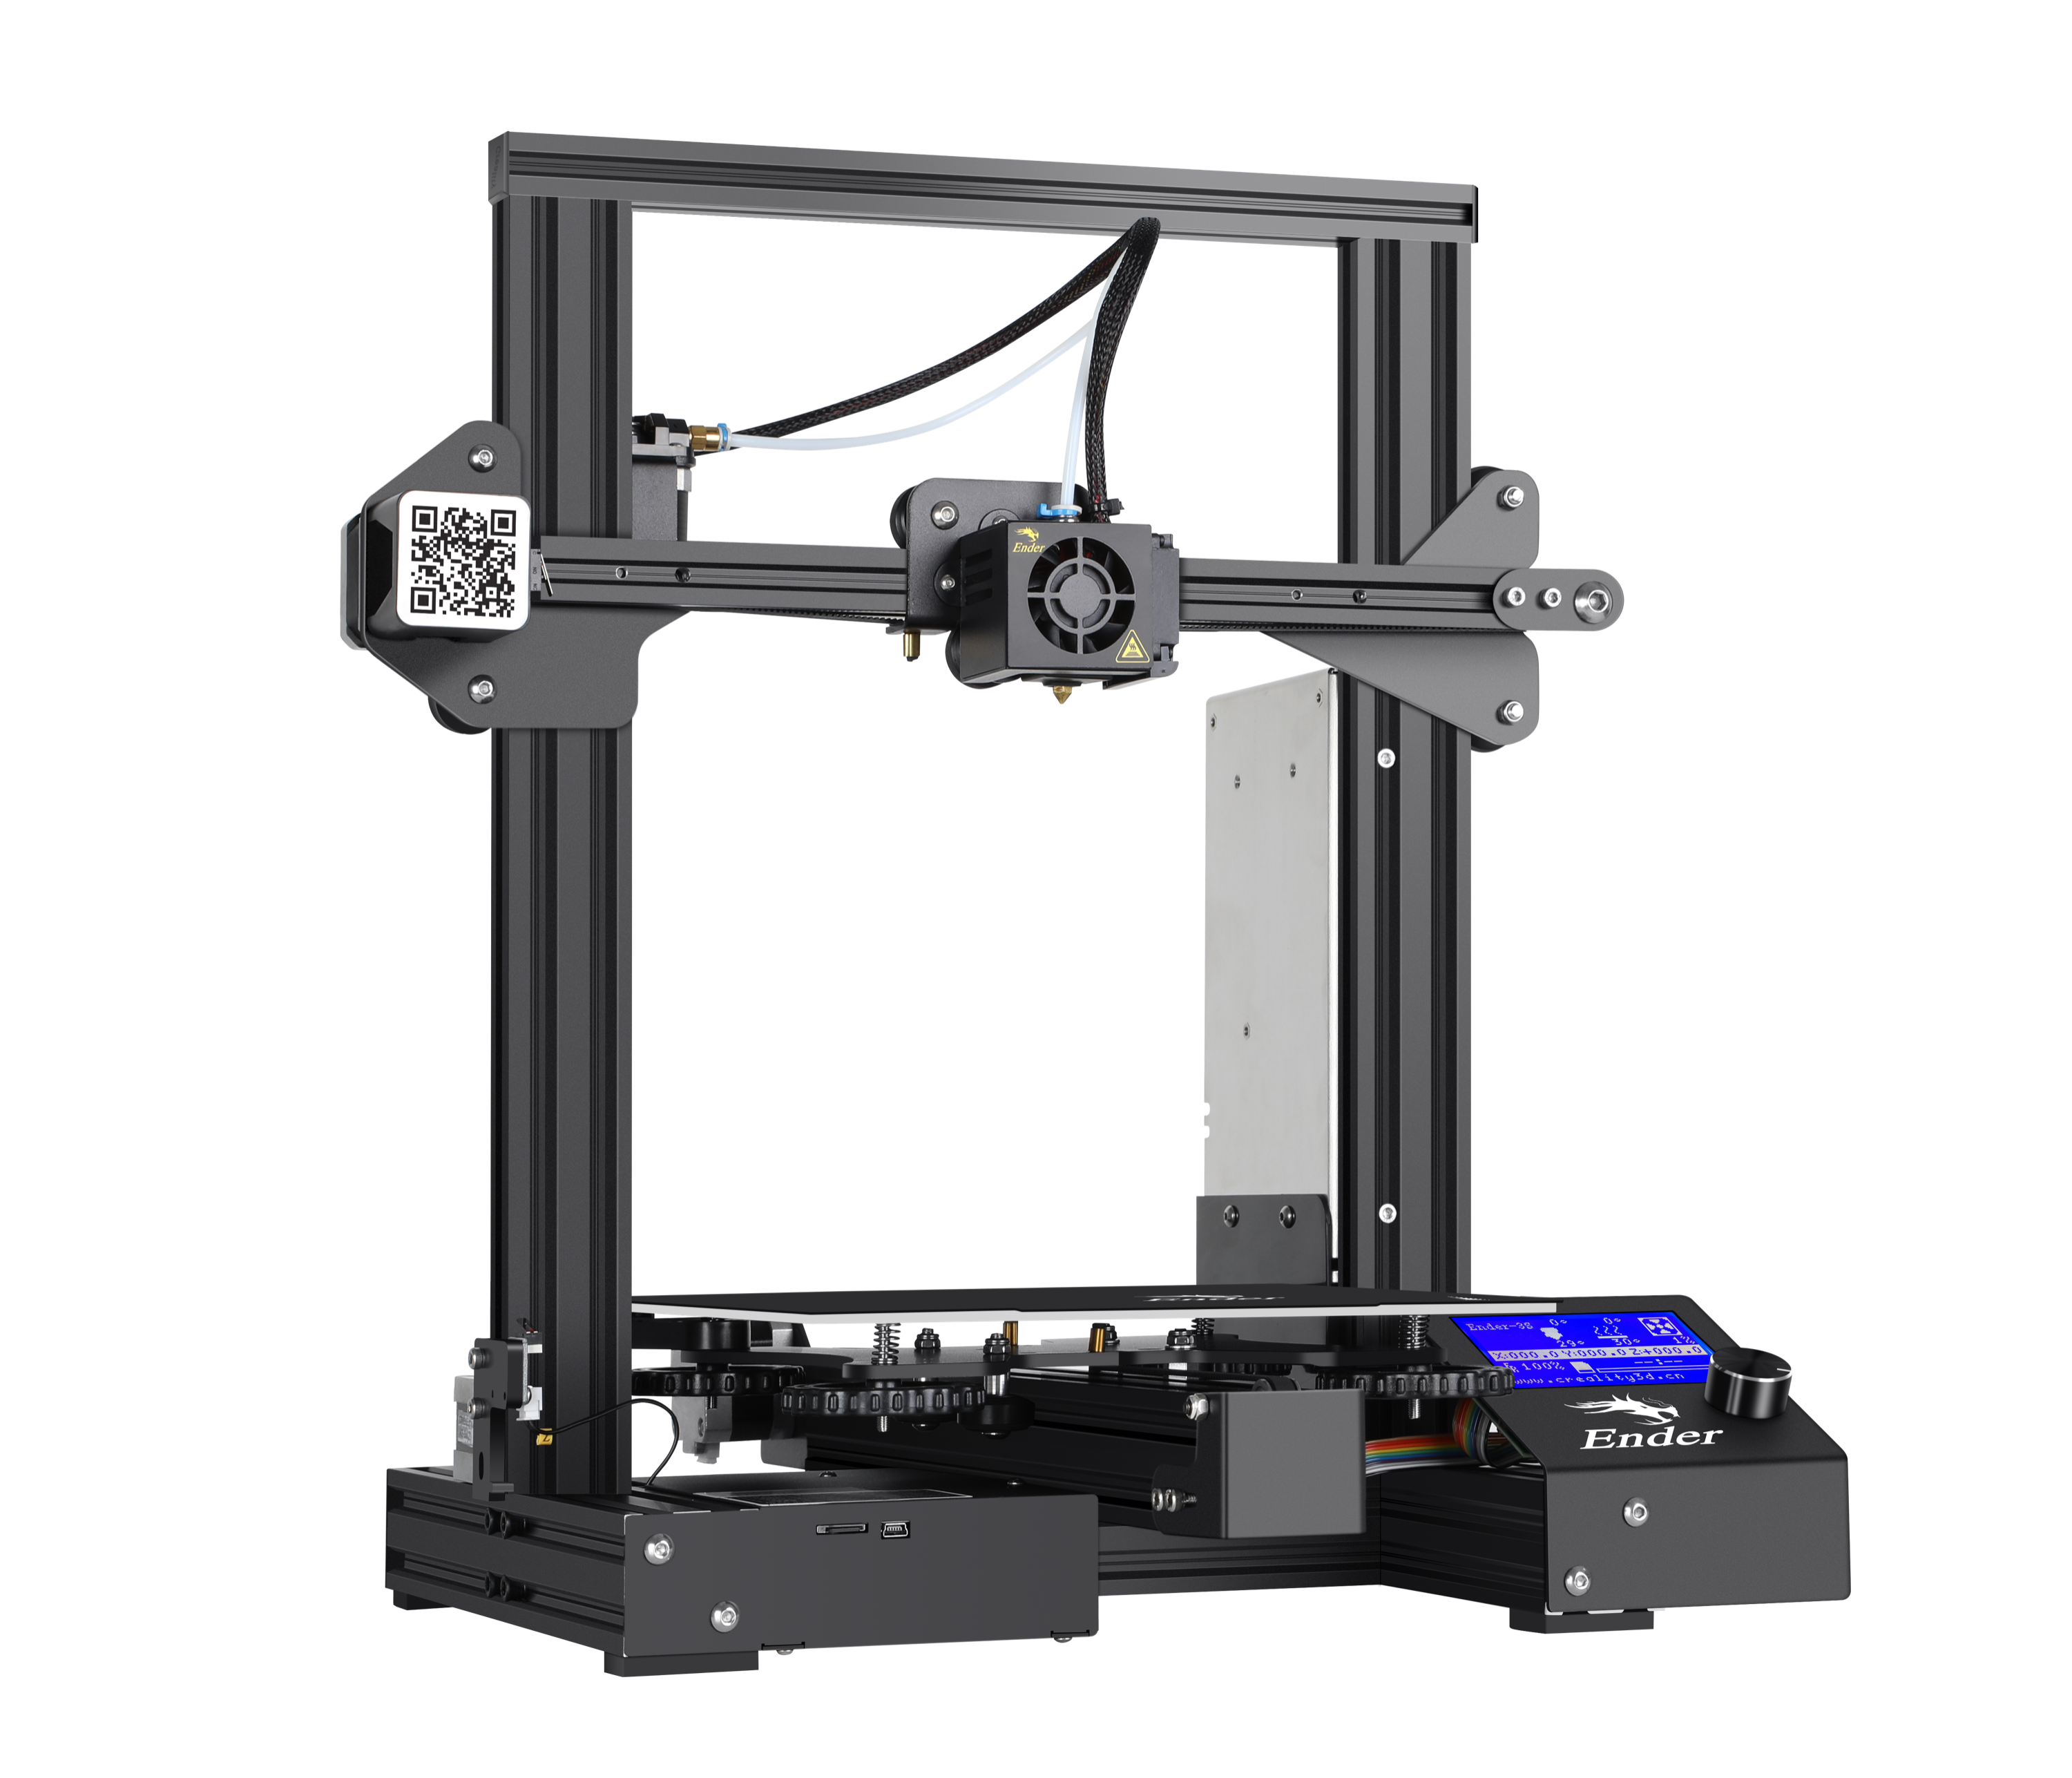
\includegraphics[width=8cm]{figs/ender3.png}
\end{center}
\caption{Ender-3 Pro V1 2017}
\label{fig:ender3pro}
\end{figure}\   

\begin{table}[H]
\begin{center}
\begin{tabular}{|c|c|c|c|}
\hline
\textbf{Componente} & \textbf{Modelo} & \textbf{Cantidad} & \textbf{Precio total} \\
\hline
Motor Nema 17 & 17HS24-2104S & 3 & 56\euro \\
Controlador & TMC2209 & 3 & 10\euro \\
Placa base & MKS DLC32 & 1 & 16\euro \\
Final de carrera & MakerBot (rojo) & 3 & 5\euro \\
Fuente de alimentación & 24V 5A (opcional)\ref{subsec:fuente_alimentacion} & 1 & 15\euro \\
Rodamiento &  F695-2RS Fushi & 22 & 15\euro \\
Rodamiento & F623RS Fushi & 6 & 5.5\euro \\
Polea GT2 & Correa:6mm ID:5mm & 3 & 1.5\euro \\
Correa GT2 & Correa:6mm Largo:252mm & 2 & 3.5\euro \\ 
Correa GT2 &  Correa:6mm Largo:280mm & 1 & 1.8\euro \\ 
Ventilador & 24V 4010 & 1 & 2\euro \\
Electroimán & D20H15mm 3KG 24V & 1 & 3\euro \\
Plástico para imprimir & PLA/PETG 1Kg & 1 & 22\euro \\
\hline
\end{tabular}
\caption{Componentes hardware necesarios}
\label{cuadro:componentes}
\end{center}
\end{table}

\begin{table}[H]
\begin{center}
\begin{tabular}{|c|c|c|}
\hline
\textbf{Componente} & \textbf{Cantidad} & \textbf{Precio total} \\
\hline
Tornillo M3 Allen & 3 & 56\euro \\

\hline
\end{tabular}
\caption{Tornillería necesaria}
\label{cuadro:tornilleria}
\end{center}
\end{table}

El precio total de los componentes necesarios es: 156.3\euro
\begin{table}[H]
\begin{center}
\begin{tabular}{|c|c|c|}
\hline
\textbf{Identificador} & \textbf{Cantidad} & \textbf{Relleno óptimo} \\
\hline
\#1 & 1 & 15\% \\
\hline
\end{tabular}
\caption{Piezas necesarias}
\label{cuadro:piezas}
\end{center}
\end{table}